% Apresentação do projeto (10 min + 5 min de arguição). Compilar com pdfLaTeX.
\documentclass[aspectratio=169,11pt]{beamer}

\usepackage[T1]{fontenc}
\usepackage[utf8]{inputenc}
\usepackage[brazil]{babel}
\usepackage{lmodern}
\usepackage{booktabs}
\usepackage{amsmath}
\usepackage{siunitx}
\sisetup{output-decimal-marker={,}, group-separator={\,}, group-minimum-digits=4, exponent-product=\times}
\usepackage{tikz}
\usetikzlibrary{positioning,calc}

% ---------------- Estilo (cores da identidade IEEE) ----------------
\definecolor{ieeeblue}{HTML}{00629B}
\definecolor{ieeedark}{HTML}{002855}
\definecolor{cinza}{HTML}{52514E}
\definecolor{pistao}{HTML}{2A78D6}
\definecolor{turboelice}{HTML}{EB6834}
\definecolor{turbofan}{HTML}{1BAF7A}

\usetheme{default}
\setbeamertemplate{navigation symbols}{}
\setbeamercolor{frametitle}{fg=white,bg=ieeeblue}
\setbeamercolor{title}{fg=ieeedark}
\setbeamercolor{structure}{fg=ieeeblue}
\setbeamercolor{normal text}{fg=black}
\setbeamercolor{alerted text}{fg=ieeeblue}
\setbeamerfont{frametitle}{size=\large,series=\bfseries}
\setbeamertemplate{itemize items}[square]
\setbeamertemplate{frametitle}{%
  \nointerlineskip
  \begin{beamercolorbox}[wd=\paperwidth,ht=8.5mm,dp=3mm,leftskip=6mm]{frametitle}
    \usebeamerfont{frametitle}\insertframetitle
  \end{beamercolorbox}}
\setbeamertemplate{footline}{%
  \hbox{\begin{beamercolorbox}[wd=\paperwidth,ht=4mm,dp=1.5mm,leftskip=6mm,rightskip=6mm]{}%
    \color{cinza}\tiny Confiabilidade de motores aeronáuticos \textbar{} Engenharia de Sistemas, UFMG%
    \hfill\insertframenumber\,/\,\inserttotalframenumber
  \end{beamercolorbox}}}
\setlength{\leftmargini}{1.2em}
\newcommand{\destaque}[1]{{\color{ieeeblue}\bfseries #1}}
\newcommand{\pcmh}{por $10^5$~h}
\newcommand{\pendente}[1]{{\color{blue}[#1]}}

\title{Análise Comparativa da Confiabilidade de Motores Aeronáuticos a Pistão, Turboélice e Turbofan}
\author{Ana Amantea Leal Marques Afonso \and Bruno Lima Soares \and Eduarda Amaral de Oliveira \and Mariana Pinho Barroso Sousa \and Victor Almeida Morais}
\institute{Engenharia de Sistemas, Universidade Federal de Minas Gerais\\Belo Horizonte, Brasil}
\date{2026}

\begin{document}

% ======================= Pessoa 1 =======================
\begin{frame}[plain]
  \begin{tikzpicture}[remember picture,overlay]
    \fill[ieeeblue] (current page.north west) rectangle ([yshift=-4mm]current page.north east);
    \fill[ieeeblue] (current page.south west) rectangle ([yshift=4mm]current page.south east);
  \end{tikzpicture}
  \vfill
  \begin{center}
    {\color{ieeedark}\LARGE\bfseries Análise Comparativa da Confiabilidade de Motores\\[1mm] Aeronáuticos a Pistão, Turboélice e Turbofan\par}
    \vspace{6mm}
    {\small Ana Amantea Leal Marques Afonso \quad Bruno Lima Soares \quad Eduarda Amaral de Oliveira\\[0.5mm]
    Mariana Pinho Barroso Sousa \quad Victor Almeida Morais\par}
    \vspace{3mm}
    {\footnotesize\color{cinza}\textit{Engenharia de Sistemas, Universidade Federal de Minas Gerais}, Belo Horizonte, Brasil\par}
  \end{center}
  \vfill
\end{frame}

\begin{frame}{Motivação e objetivos}
  \begin{columns}[T]
    \begin{column}{0.5\textwidth}
      \textbf{O problema}
      \begin{itemize}
        \item Em um monomotor, a falha do motor em voo elimina toda a propulsão
        \item Literatura: pistão com \destaque{10 a 100} falhas \pcmh; turbinas abaixo de \destaque{1}
        \item Mas é uma \emph{taxa única} para o motor inteiro: não diz onde estão as falhas nem se a redundância compensa
      \end{itemize}
    \end{column}
    \begin{column}{0.47\textwidth}
      \textbf{Objetivos}
      \begin{enumerate}
        \item Representar cada motor em um diagrama de blocos de confiabilidade (RBD)
        \item Estimar $\lambda$, MTBF e $R(t)$
        \item Avaliar redundâncias: magnetos, FADEC de dois canais e \emph{dois motores}
        \item Identificar os subsistemas mais críticos
      \end{enumerate}
    \end{column}
  \end{columns}
\end{frame}

\begin{frame}{Um problema de Engenharia de Sistemas}
  \begin{columns}[c]
    \begin{column}{0.42\textwidth}
      \centering
      \begin{tikzpicture}[
        nivel/.style={draw=ieeeblue, fill=ieeeblue!8, rounded corners=2pt, text width=36mm, minimum height=8mm, align=center, font=\footnotesize},
        nota/.style={font=\scriptsize\color{cinza}, align=center},
        >=stealth, line width=0.5pt]
        \node[nivel] (a) at (0,0) {\textbf{Aeronave}\\[-0.5mm]{\scriptsize um ou dois motores?}};
        \node[nivel] (m) at (0,-1.25) {\textbf{Motor}\\[-0.5mm]{\scriptsize arquitetura em RBD}};
        \node[nivel] (s) at (0,-2.5) {\textbf{Subsistemas}\\[-0.5mm]{\scriptsize série e pares redundantes}};
        \node[nivel] (c) at (0,-3.75) {\textbf{Componentes}\\[-0.5mm]{\scriptsize falhas em operação}};
        \draw[->] (a) -- (m); \draw[->] (m) -- (s); \draw[->] (s) -- (c);
        \draw[->, ieeeblue, line width=0.8pt] ([xshift=2mm]c.south east) -- node[midway, sloped, below, font=\scriptsize] {integração: a confiabilidade emerge} ([xshift=2mm]a.north east);
        \draw[->, cinza] ([xshift=-2mm]a.north west) -- node[midway, sloped, below, font=\scriptsize] {decomposição} ([xshift=-2mm]c.south west);
      \end{tikzpicture}
    \end{column}
    \begin{column}{0.56\textwidth}
      \small
      \begin{itemize}
        \item \textbf{Fronteira e requisito}: o evento de falha é não entregar a potência exigida; tanques e erro do piloto ficam fora do sistema
        \item \textbf{Confiabilidade é propriedade emergente}: depende de como os subsistemas se arranjam (série $\times$ paralelo), não só de cada peça
        \item \textbf{Trade-off de arquitetura}: redundância compensa uma tecnologia pior? Depende da causa comum entre as partes ($\beta$)
        \item \textbf{Ciclo de vida}: dados de operação e manutenção voltam para o projeto e apontam onde intervir
      \end{itemize}
    \end{column}
  \end{columns}
\end{frame}

\begin{frame}{O que a literatura já oferece}
  \begin{columns}[T]
    \begin{column}{0.48\textwidth}
      \textbf{Técnicas}
      \begin{itemize}
        \item FMEA, FTA e RBD em propulsão, com pouca informação de campo (NASA, 2000)
        \item RBD em série de um turboeixo a partir de registros de campo (Samuel \emph{et al.}, 2006)
        \item Fator $\beta$ para causa comum (Ebeling, 1997)
      \end{itemize}
    \end{column}
    \begin{column}{0.48\textwidth}
      \textbf{Dados}
      \begin{itemize}
        \item ATSB: taxas medidas para motores a pistão
        \item Turbinas: em geral \emph{limites} regulatórios (ETOPS, SET-IMC), que dizem quanto o motor pode falhar, não quanto falha
        \item NTSB: achados por componente e horas do motor, mas \emph{sem horas voadas da frota}
      \end{itemize}
    \end{column}
  \end{columns}
  \vspace{1mm}
  \begin{center}
    \fcolorbox{ieeeblue}{white}{\parbox{0.85\textwidth}{\centering\small Lacuna: nenhum estudo compara as três tecnologias dentro do mesmo modelo.}}
  \end{center}
\end{frame}

% ======================= Pessoa 2 =======================
\begin{frame}{Sistema estudado: três motores, três RBD}
  \centering
  {\small Lycoming O-540 (pistão) \quad\textbar\quad PT6A-34 (turboélice) \quad\textbar\quad CFM56-7B (turbofan)\par}
  \vspace{1.5mm}
  \makebox[\linewidth]{\resizebox{0.97\paperwidth}{!}{% Diagramas de blocos de confiabilidade (RBD) dos três motores. Blocos empilhados: par redundante.
\begin{tikzpicture}[
  font=\fontsize{7}{8}\selectfont,
  blk/.style={draw, rounded corners=1pt, align=center, minimum height=6.6mm, inner sep=1.5pt, text width=#1},
  blk/.default=12mm,
  rot/.style={font=\footnotesize\bfseries, anchor=east},
  >=stealth, line width=0.4pt]
\def\g{2.2mm}
% ---------------- Pistão ----------------
\node[rot] (lp) at (0,0) {Pistão};
\node[blk=11mm, right=\g of lp] (p1) {Admissão};
\coordinate[right=\g of p1] (p2i);
\node[blk=11mm, right=\g of p2i, yshift=4.6mm] (p2a) {Bomba mecânica};
\node[blk=11mm, right=\g of p2i, yshift=-4.6mm] (p2b) {Bomba elétrica};
\coordinate (p2o) at ($(p2a.east |- p2i)+(\g,0)$);
\node[blk=13mm, right=\g of p2o] (p3) {Carburador / injeção};
\coordinate[right=\g of p3] (p4i);
\node[blk=11mm, right=\g of p4i, yshift=4.6mm] (p4a) {Magneto 1};
\node[blk=11mm, right=\g of p4i, yshift=-4.6mm] (p4b) {Magneto 2};
\coordinate (p4o) at ($(p4a.east |- p4i)+(\g,0)$);
\node[blk=19mm, right=\g of p4o] (p5) {Cilindros, válvulas, pistões, virabrequim};
\node[blk=13mm, right=\g of p5] (p6) {Lubrificação};
\node[blk=15.5mm, right=\g of p6] (p7) {Arrefecimento};
\node[blk=13.5mm, right=\g of p7] (p8) {Hélice e governador};
\draw (p1) -- (p2i) |- (p2a); \draw (p2i) |- (p2b);
\draw (p2a) -| (p2o); \draw (p2b) -| (p2o); \draw (p2o) -- (p3);
\draw (p3) -- (p4i) |- (p4a); \draw (p4i) |- (p4b);
\draw (p4a) -| (p4o); \draw (p4b) -| (p4o); \draw (p4o) -- (p5);
\draw (p5) -- (p6) -- (p7) -- (p8);
% ---------------- Turboélice ----------------
\node[rot] (lt) at (0,-1.75) {Turboélice};
\node[blk=10mm, right=\g of lt] (t1) {Entrada de ar};
\node[blk=13mm, right=\g of t1] (t2) {Compressor};
\node[blk=13mm, right=\g of t2] (t3) {Câmara de combustão};
\node[blk=17mm, right=\g of t3] (t4) {Turbinas (compressor e livre)};
\node[blk=11mm, right=\g of t4] (t5) {Caixa de redução};
\node[blk=13.5mm, right=\g of t5] (t6) {Hélice e governador};
\node[blk=13mm, right=\g of t6] (t7) {Combustível (FCU)};
\node[blk=13mm, right=\g of t7] (t8) {Lubrificação};
\draw (t1) -- (t2) -- (t3) -- (t4) -- (t5) -- (t6) -- (t7) -- (t8);
% ---------------- Turbofan ----------------
\node[rot] (lf) at (0,-3.35) {Turbofan};
\node[blk=7mm, right=\g of lf] (f1) {Fan};
\node[blk=15.5mm, right=\g of f1] (f2) {Compressores LP e HP};
\node[blk=13mm, right=\g of f2] (f3) {Câmara de combustão};
\node[blk=12mm, right=\g of f3] (f4) {Turbinas HP e LP};
\coordinate[right=\g of f4] (f5i);
\node[blk=11mm, right=\g of f5i, yshift=4.6mm] (f5a) {FADEC A};
\node[blk=11mm, right=\g of f5i, yshift=-4.6mm] (f5b) {FADEC B};
\coordinate (f5o) at ($(f5a.east |- f5i)+(\g,0)$);
\node[blk=13mm, right=\g of f5o] (f6) {Combustível};
\node[blk=13mm, right=\g of f6] (f7) {Lubrificação};
\node[blk=12mm, right=\g of f7] (f8) {Caixa de acessórios};
\draw (f1) -- (f2) -- (f3) -- (f4) -- (f5i) |- (f5a); \draw (f5i) |- (f5b);
\draw (f5a) -| (f5o); \draw (f5b) -| (f5o); \draw (f5o) -- (f6) -- (f7) -- (f8);
\end{tikzpicture}
}}
  \vspace{1mm}
  {\footnotesize\raggedright
  Falha = perda de potência que obriga a desligar o motor. Bloco em série: sua falha derruba o motor. Blocos empilhados: par redundante, que só falha se as duas unidades falharem.\par}
\end{frame}

\begin{frame}{Método: taxa da literatura, frações medidas}
  \begin{columns}[T]
    \begin{column}{0.52\textwidth}
      \small
      \textbf{Modelo} (taxa constante)
      \begin{itemize}
        \item Série: $R_s = \prod_i e^{-\lambda_i t}$
        \item Par com causa comum $\beta$:
          \[ R_p = \left[1-\left(1-e^{-(1-\beta)\lambda_u t}\right)^2\right] e^{-\beta\lambda_u t} \]
        \item Distribuição da taxa: $\lambda_i = \lambda_s\, n_i/N_s$
        \item Unidade do par: $\lambda_u = n_p\lambda/(2N_s)$
        \item Taxa publicada preservada em um voo de 1~h
      \end{itemize}
    \end{column}
    \begin{column}{0.45\textwidth}
      \small
      \textbf{Dados}
      \begin{center}
      \begin{tabular}{@{}lrr@{}}
        \toprule
        NTSB, 2008--2026 & Falhas & Registros \\
        \midrule
        Pistão & 2562 & 994 \\
        Turboélice & 176 & 69 \\
        Turbofan & 161 & 46 \\
        \midrule
        Total & 2899 & \destaque{1109} \\
        \bottomrule
      \end{tabular}
      \end{center}
      \begin{itemize}
        \item Falha: perda de potência na sequência de eventos; pane seca à parte
        \item Bloco: código ATA do achado (ex.: 8530 cilindros, 7414 magneto)
        \item $\lambda$ nominal: 12,4; 0,15; 0,20 \pcmh
      \end{itemize}
    \end{column}
  \end{columns}
\end{frame}

% ======================= Pessoa 3 =======================
\begin{frame}{Resultado 1: o pistão falha 62 a 83 vezes mais}
  \begin{columns}[c]
    \begin{column}{0.53\textwidth}
      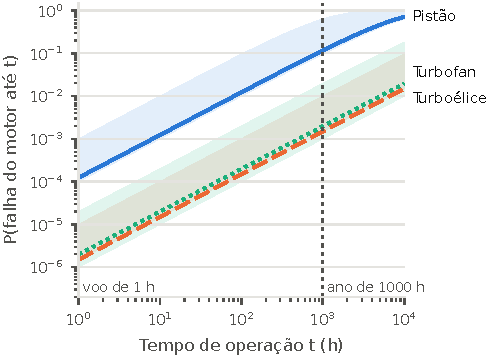
\includegraphics[width=\textwidth]{figures/fig_prob_falha_tempo}
    \end{column}
    \begin{column}{0.45\textwidth}
      \small
      \begin{tabular}{@{}lcc@{}}
        \toprule
        Motor & $F(1\,\mathrm{h})$ & $R(1000\,\mathrm{h})$ \\
        \midrule
        Pistão & \num{1.24e-4} & 0,883 \\
        Turboélice & \num{1.5e-6} & 0,9985 \\
        Turbofan & \num{2.0e-6} & 0,9980 \\
        \bottomrule
      \end{tabular}
      \vspace{2mm}
      \begin{itemize}
        \item Em 1000~h: \destaque{12\%} de chance de falha no pistão, 0,15--0,20\% nas turbinas
        \item No pior caso das faixas, o pistão ainda falha \destaque{5 vezes} mais
        \item Turboélice $\times$ turbofan: faixas sobrepostas, \emph{sem ordem}
      \end{itemize}
    \end{column}
  \end{columns}
\end{frame}

\begin{frame}{Resultado 2: onde as falhas se concentram}
  \centering
  \resizebox{\textwidth}{!}{\begin{tikzpicture}% Gerado de saida/tabelas/pareto_blocos.csv: cinco maiores blocos por motor
% (parcela na falha em 1 h; traço: IC de Jeffreys de 95%). Escala: 100% = 3.0 cm.
\node[anchor=west,font=\small\bfseries,text=pistao] at (0.00,0.8) {Pistão};
\node[anchor=east,align=right,text width=2.9cm,font=\scriptsize\linespread{0.85}\selectfont] at (2.92,-0.00) {Cilindros, válvulas, pistões, virabrequim};
\fill[pistao] (3.000,-0.20) rectangle (4.802,0.20);
\draw[black!65,line width=0.5pt] (4.705,-0.00) -- (4.897,-0.00);
\node[anchor=west,font=\scriptsize] at (4.897,-0.00) {60\%};
\node[anchor=east,align=right,text width=2.9cm,font=\scriptsize\linespread{0.85}\selectfont] at (2.92,-0.72) {Lubrificação};
\fill[pistao] (3.000,-0.92) rectangle (3.430,-0.52);
\draw[black!65,line width=0.5pt] (3.364,-0.72) -- (3.503,-0.72);
\node[anchor=west,font=\scriptsize] at (3.503,-0.72) {14\%};
\node[anchor=east,align=right,text width=2.9cm,font=\scriptsize\linespread{0.85}\selectfont] at (2.92,-1.44) {Carburador / injeção};
\fill[pistao] (3.000,-1.64) rectangle (3.410,-1.24);
\draw[black!65,line width=0.5pt] (3.346,-1.44) -- (3.481,-1.44);
\node[anchor=west,font=\scriptsize] at (3.481,-1.44) {14\%};
\node[anchor=east,align=right,text width=2.9cm,font=\scriptsize\linespread{0.85}\selectfont] at (2.92,-2.16) {Admissão};
\fill[pistao] (3.000,-2.36) rectangle (3.203,-1.96);
\draw[black!65,line width=0.5pt] (3.158,-2.16) -- (3.257,-2.16);
\node[anchor=west,font=\scriptsize] at (3.257,-2.16) {7\%};
\node[anchor=east,align=right,text width=2.9cm,font=\scriptsize\linespread{0.85}\selectfont] at (2.92,-2.88) {Hélice e governador};
\fill[pistao] (3.000,-3.08) rectangle (3.122,-2.68);
\draw[black!65,line width=0.5pt] (3.087,-2.88) -- (3.166,-2.88);
\node[anchor=west,font=\scriptsize] at (3.166,-2.88) {4\%};
\node[anchor=west,font=\small\bfseries,text=turboelice] at (5.55,0.8) {Turboélice};
\node[anchor=east,align=right,text width=2.9cm,font=\scriptsize\linespread{0.85}\selectfont] at (8.47,-0.00) {Turbinas (compressor e livre)};
\fill[turboelice] (8.550,-0.20) rectangle (9.507,0.20);
\draw[black!65,line width=0.5pt] (9.204,-0.00) -- (9.853,-0.00);
\node[anchor=west,font=\scriptsize] at (9.853,-0.00) {32\%};
\node[anchor=east,align=right,text width=2.9cm,font=\scriptsize\linespread{0.85}\selectfont] at (8.47,-0.72) {Compressor};
\fill[turboelice] (8.550,-0.92) rectangle (9.159,-0.52);
\draw[black!65,line width=0.5pt] (8.914,-0.72) -- (9.476,-0.72);
\node[anchor=west,font=\scriptsize] at (9.476,-0.72) {20\%};
\node[anchor=east,align=right,text width=2.9cm,font=\scriptsize\linespread{0.85}\selectfont] at (8.47,-1.44) {Combustível (FCU)};
\fill[turboelice] (8.550,-1.64) rectangle (9.028,-1.24);
\draw[black!65,line width=0.5pt] (8.813,-1.44) -- (9.327,-1.44);
\node[anchor=west,font=\scriptsize] at (9.327,-1.44) {16\%};
\node[anchor=east,align=right,text width=2.9cm,font=\scriptsize\linespread{0.85}\selectfont] at (8.47,-2.16) {Lubrificação};
\fill[turboelice] (8.550,-2.36) rectangle (8.941,-1.96);
\draw[black!65,line width=0.5pt] (8.750,-2.16) -- (9.224,-2.16);
\node[anchor=west,font=\scriptsize] at (9.224,-2.16) {13\%};
\node[anchor=east,align=right,text width=2.9cm,font=\scriptsize\linespread{0.85}\selectfont] at (8.47,-2.88) {Hélice e governador};
\fill[turboelice] (8.550,-3.08) rectangle (8.854,-2.68);
\draw[black!65,line width=0.5pt] (8.690,-2.88) -- (9.117,-2.88);
\node[anchor=west,font=\scriptsize] at (9.117,-2.88) {10\%};
\node[anchor=west,font=\small\bfseries,text=turbofan] at (11.10,0.8) {Turbofan};
\node[anchor=east,align=right,text width=2.9cm,font=\scriptsize\linespread{0.85}\selectfont] at (14.02,-0.00) {Compressores LP e HP};
\fill[turbofan] (14.100,-0.20) rectangle (15.299,0.20);
\draw[black!65,line width=0.5pt] (14.899,-0.00) -- (15.735,-0.00);
\node[anchor=west,font=\scriptsize] at (15.735,-0.00) {40\%};
\node[anchor=east,align=right,text width=2.9cm,font=\scriptsize\linespread{0.85}\selectfont] at (14.02,-0.72) {Turbinas HP e LP};
\fill[turbofan] (14.100,-0.92) rectangle (14.899,-0.52);
\draw[black!65,line width=0.5pt] (14.564,-0.72) -- (15.321,-0.72);
\node[anchor=west,font=\scriptsize] at (15.321,-0.72) {27\%};
\node[anchor=east,align=right,text width=2.9cm,font=\scriptsize\linespread{0.85}\selectfont] at (14.02,-1.44) {Combustível};
\fill[turbofan] (14.100,-1.64) rectangle (14.633,-1.24);
\draw[black!65,line width=0.5pt] (14.363,-1.44) -- (15.022,-1.44);
\node[anchor=west,font=\scriptsize] at (15.022,-1.44) {18\%};
\node[anchor=east,align=right,text width=2.9cm,font=\scriptsize\linespread{0.85}\selectfont] at (14.02,-2.16) {Caixa de acessórios};
\fill[turbofan] (14.100,-2.36) rectangle (14.366,-1.96);
\draw[black!65,line width=0.5pt] (14.192,-2.16) -- (14.692,-2.16);
\node[anchor=west,font=\scriptsize] at (14.692,-2.16) {9\%};
\node[anchor=east,align=right,text width=2.9cm,font=\scriptsize\linespread{0.85}\selectfont] at (14.02,-2.88) {Câmara de combustão};
\fill[turbofan] (14.100,-3.08) rectangle (14.233,-2.68);
\draw[black!65,line width=0.5pt] (14.128,-2.88) -- (14.505,-2.88);
\node[anchor=west,font=\scriptsize] at (14.505,-2.88) {4\%};
\end{tikzpicture}}
  \vspace{1.5mm}
  \begin{columns}[T]
    \begin{column}{0.48\textwidth}
      \small
      \begin{itemize}
        \item Pistão: núcleo mecânico com \destaque{60\%}; os 5 blocos em série sem redundância somam 99\%
        \item Magnetos duplicados: só 0,6\%
      \end{itemize}
    \end{column}
    \begin{column}{0.48\textwidth}
      \small
      \begin{itemize}
        \item Turbinas: compressores e turbinas lideram (\destaque{52\%} no turboélice, \destaque{67\%} no turbofan)
        \item Poucos registros (69 e 45): intervalos largos
      \end{itemize}
    \end{column}
  \end{columns}
\end{frame}

% ======================= Pessoa 4 =======================
\begin{frame}{Resultado 3: redundância dentro do motor}
  \centering
  \begin{tabular}{@{}lrrcr@{}}
    \toprule
    Par & Registros & $\lambda_u$ (\pcmh) & Ganho & Sem o par \\
    \midrule
    Magnetos (pistão) & 102 & 0,72 & 10$\times$ & +5,2\% \\
    Bombas (pistão) & 12 & 0,085 & 10$\times$ & +0,6\% \\
    FADEC A/B (turbofan) & 1 & 0,0022 & 10$\times$ & +1,0\% \\
    \bottomrule
  \end{tabular}
  \vspace{5mm}
  \begin{itemize}
    \item Ganho: $F$ de uma unidade sobre $F$ do par. Sem o par: aumento em $F(1\,\mathrm{h})$ do motor
    \item O par reduz em cerca de \destaque{10 vezes} a chance de perder a função, e esse ganho é limitado pela causa comum: fica perto de $1/\beta$, com $\beta = 0{,}1$
    \item Sem os dois pares, o pistão falharia \destaque{5,8\%} mais em 1~h
    \item O mesmo número é o risco de decolar com um magneto já em pane: +5,2\%
    \item FADEC: um único registro no NTSB; falhas que o par tolera raramente viram acidente
  \end{itemize}
\end{frame}

\begin{frame}{Resultado 4: dois pistões $\times$ uma turbina}
  \begin{columns}[c]
    \begin{column}{0.53\textwidth}
      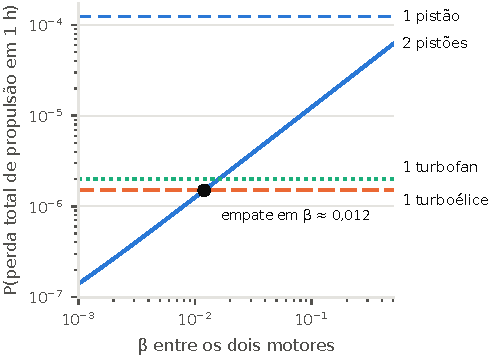
\includegraphics[width=\textwidth]{figures/fig_bimotor}
    \end{column}
    \begin{column}{0.45\textwidth}
      \small
      \begin{itemize}
        \item Falhas independentes: perda total em \num{1.5e-8} por hora
        \item Mas a causa comum entre motores (combustível, manutenção, gelo) domina
        \item Empate em \destaque{$\beta = 0{,}012$} contra o turboélice e \destaque{$0{,}016$} contra o turbofan
        \item A faixa usual de $\beta$ vai de 0,01 a 0,3
        \item O bimotor ainda \emph{dobra} a chance de alguma falha de motor no voo
      \end{itemize}
    \end{column}
  \end{columns}
\end{frame}

% ======================= Pessoa 5 =======================
\begin{frame}{Resultado 5: o que dizem as ocorrências do NTSB}
  \begin{columns}[c]
    \begin{column}{0.55\textwidth}
      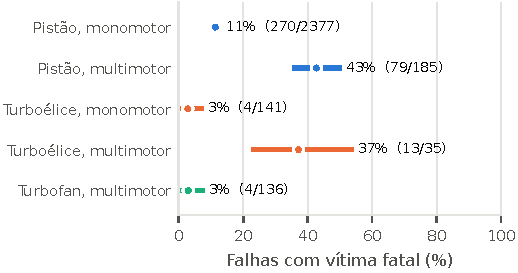
\includegraphics[width=\textwidth]{figures/fig_ntsb_prob_fatal}
    \end{column}
    \begin{column}{0.43\textwidth}
      \small
      \begin{itemize}
        \item Falhas de motor com vítima fatal, 2008--2026
        \item Pistão: \destaque{43\%} nos multimotores contra 11\% nos monomotores
        \item Turboélice monomotor: \destaque{2,8\%}, perto do turbofan (2,9\%)
        \item Falha de um motor no multimotor que chega ao NTSB é das mais graves: perda de controle com tração assimétrica
        \item Ressalva: no multimotor, a falha que termina em pouso normal quase não entra na base
      \end{itemize}
    \end{column}
  \end{columns}
\end{frame}

\begin{frame}{Limitações}
  \begin{itemize}
    \item \textbf{Frações por contagem}: supõem a mesma chance de registro para todos os blocos; o NTSB vê sobretudo acidentes (2529 das 2562 falhas no pistão)
    \item \textbf{Poucos dados nas turbinas}: 69 e 45 registros; motores por tipo, não por modelo; 535 achados genéricos fora da contagem
    \item \textbf{Taxa constante}: caso-controle pelo TSO dá forma 0,99 (IC de 0,94 a 1,05; 903 falhas), mas supõe que os controles tenham a idade da frota
    \item \textbf{Sem horas voadas}: a atualização Gama--Poisson das taxas absolutas não foi possível
    \item \textbf{Taxa do turbofan}: vem do fabricante, sem estatística independente
  \end{itemize}
\end{frame}

\begin{frame}{Conclusões}
  \begin{itemize}
    \item O pistão falha \destaque{62 a 83 vezes} mais que as turbinas, e a diferença resiste a toda a faixa da literatura
    \item As falhas do pistão estão no \destaque{núcleo mecânico}, sem redundância; é ali que manutenção e projeto rendem mais
    \item \destaque{Redundância não compensa tecnologia}: dois pistões só superam uma turbina com $\beta$ abaixo de 1,2--1,6\%, e o NTSB confirma
    \item Lição de sistemas: a escolha de arquitetura só se avalia com as \emph{dependências} entre as partes; ignorar a causa comum superestima o ganho da redundância
    \item Turboélice $\times$ turbofan: os dados publicados não permitem ordenar
  \end{itemize}
  \vspace{3mm}
  \textbf{Próximos passos}: obter horas voadas por frota, ampliar a base das turbinas e usar remoções em campo como limite superior de $\lambda_u$.
\end{frame}

\begin{frame}[plain]
  \begin{tikzpicture}[remember picture,overlay]
    \fill[ieeeblue] (current page.north west) rectangle ([yshift=-4mm]current page.north east);
    \fill[ieeeblue] (current page.south west) rectangle ([yshift=4mm]current page.south east);
  \end{tikzpicture}
  \vfill
  \begin{center}
    {\color{ieeedark}\Huge\bfseries Obrigado!\par}
    \vspace{4mm}
    {\large Perguntas?\par}
  \end{center}
  \vfill
\end{frame}

% ======================= Apoio para a arguição =======================
\appendix
\begin{frame}{Apoio: sensibilidade, blocos sem registro e Weibull}
  \small
  \begin{columns}[T]
    \begin{column}{0.48\textwidth}
      \textbf{Sensibilidade} (mínimo a máximo de cada parâmetro)
      \begin{itemize}
        \item Taxa total: $F(1\,\mathrm{h})$ varia 10$\times$ (pistão), 6,7$\times$ (turboélice) e 20$\times$ (turbofan)
        \item $\beta$ e $\lambda_u$: não mudam $F(1\,\mathrm{h})$, porque a taxa publicada é preservada; só redistribuem o Pareto
      \end{itemize}
      \textbf{Blocos sem registro}
      \begin{itemize}
        \item Lubrificação do turbofan e entrada de ar do turboélice: fração 0
        \item Zero registros não é taxa zero: o limite de Jeffreys vai a 5\% e 4\%
      \end{itemize}
    \end{column}
    \begin{column}{0.48\textwidth}
      \textbf{Forma de Weibull} (caso-controle, monomotores)
      \begin{itemize}
        \item Pistão, TSO: 0,99 (0,94--1,05), $p=0{,}79$: taxa constante
        \item Pistão, TSN: 1,08 (1,02--1,13): desgaste leve na vida do motor
        \item Turboélice, TSO: 1,28 (0,97--1,59), só 32 falhas
      \end{itemize}
      \textbf{Combustível, contado à parte}
      \begin{itemize}
        \item Pistão: 1532 ocorrências, 174 com vítima fatal
      \end{itemize}
    \end{column}
  \end{columns}
\end{frame}

\end{document}
